At first sight, the key findings discussed by Frantz and 
Kendall-Taylor seem to hold, but further critical 
evaluation of key statistical assumptions, predictive 
accuracy and model parsimony are necessary. Following a 
brief summary of the results each point will be 
briefly discussed in the following.

\begin{figure}[!ht]
  \centering
  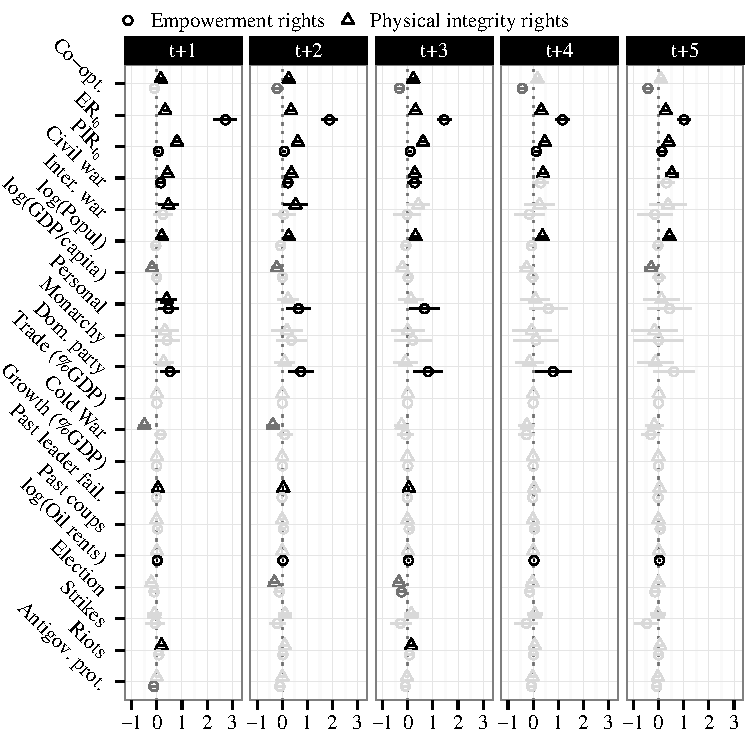
\includegraphics[width=\linewidth]{./sections/03replication/coefPlotOriginal.pdf}
  \caption{How co-optation affects political repression.
    Confidence intervals at the .95 level, positive 
    coefficients black, negative estimates grey, statistically
    insignificant results faded. Cubic polynomials and 
    cut points not shown.%
  }
  \label{fig:coefPlot}
\end{figure}

Figure \ref{fig:coefPlot} summarizes all ordered logistic
regressions presented in the original publication. 
Differences between the published and the replicated 
analyses are often negligible. With few exceptions 
coefficients and cluster robust standard errors 
agree up to two decimal places.\footnote{A more fundamental
difference concerns the polynomials on length of tenure. The 
models would not converge in $R$ unless multicollinearity 
was reduced by constructing orthogonal-polynomial 
regressors.} As can be seen from the top row in 
Figure \ref{fig:coefPlot} higher levels of co-optation 
concur with lower levels of empowerment rights 
restrictions, but they tend to go hand in hand with 
increases in physical integrity violations. Moreover, in 
line with the idea of inert government practices the 
attenuating impact of co-optation on empowerment rights 
restrictions increases in absolute size when moving from
$t+1$ to $t+5$. The same time-dependent dynamic is not 
observable for physical integrity violations. Finally, all 
models speak to the staying power of political repression 
because all lagged dependent variables are positively 
signed and statistically significant.\footnote{Why 
Erica Frantz and Andrea Kendall-Taylor regard all lagged 
reponses as continuous and treat all leads as ordinal 
variables is not clear from the paper.} In short, all
key findings can be reproduced and further evaluation of the
original publication is possible.

\begin{table}[!htb]
\centering
\caption{Parallel-regressions assumption: $\chi^2$-comparisons}
\label{tbl:Chi2comparisons}
  \begin{tabular}{ll*{5}{c}} \toprule
    ~ & ~ & $t+1$ & $t+2$ & $t+3$ & $t+4$ & $t+5$ \\ \cmidrule{2-7}
    \multirow{2}{*}{Empowerment rights} & Unadj. P-value & 1.000 & 0.499 & 0.000 & 0.000 & 0.000 \\
    ~ & Bonf. adj. P-value & 1.000 & 0.833 & 0.000 & 0.000 & 0.000 \\
    \multirow{2}{*}{Physical integrity} & Unadj. P-value & 0.003 & 0.002 & 0.000 & 0.000 & 0.000 \\
    ~ & Bonf. adj. P-value & 0.077 & 0.052 & 0.001 & 0.000 & 0.000 \\ 
    \bottomrule
    \multicolumn{7}{l}{\textit{Note:} P-values were averaged over all imputed models.} \\
  \end{tabular}
\end{table}

\begin{wrapfigure}{r}{0.45\textwidth}
\centering
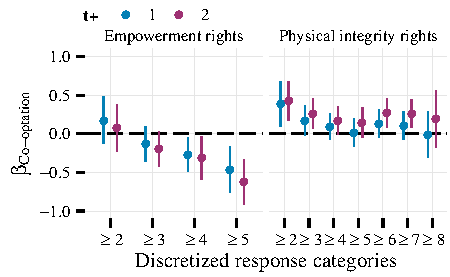
\includegraphics[width=\linewidth]{./sections/03replication/parallelRegressionsCoefPlot.pdf}
\caption{Blabla}
\label{fig:separateLogisticCoef}
\end{wrapfigure}
The parallel-regressions assumption is crucial to 
ordered logistic regression. It constraints differences 
between the cumulative distribution functions of any two 
categories to a a constant \citep[476]{Fox.2008}. In other 
the words, the slope of those curves must remain constant 
and hence the ordered logistic regression constraints all 
coefficients to equality between any two categories. One 
possibility to test this assumption is a $\chi^2$-comparison
of the constrained coefficients to their unconstrained 
alternatives from a multinomial regression. As shown in 
Table \ref{tbl:Chi2comparisons} only the four models 
predicting political repression at $t+1$ and $t+2$ reject 
the alternative hypothesis of non-constant coefficients and
thus support the statistical model. However, since the null 
hypothesis is saved only by very conservative Bonferroni 
adjusted P-values a closer look at the four supported
models seems justfied. To that end $j-1$ separate logistic 
regressions are fit to the set $\mathbbm{1}_y(y_{i} \ge j)$
of binary responses. If the parallel regressions 
assumption holds the coefficients should differ little as 
$j$ increases. Figure \ref{fig:separateLogisticCoef} shows 
the results for the key regressor co-optation. While the 
right-hand panel raises little reason for concern, 
coefficients in the left-hand panel exhibit a clear trend. 
Thus, the majority of models fails the parallel-regressions 
assumption outright and even where it holds immediately doubt
is advised.





